% !TEX root = ../../../main.tex
% 来源：高中物理甲种本·第二册（热学·电学）
% 章节：分子运动论基础 / 物体是由分子组成的
% 原始文件：1.tex，行 84-102
% 类型：tikz
% ---
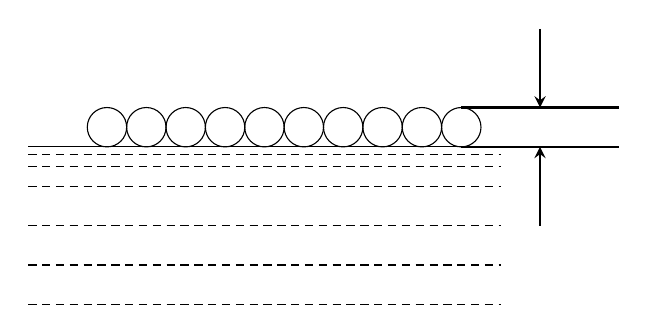
\begin{tikzpicture}[>=stealth]
\draw (0,0)--(6,0);

\foreach \x in {-.1, -.25, -.5, -1, -1.5, -2}
{ 
   \draw [densely dashed](0,\x)--(6,\x);
}

\foreach \y in {1,2,...,10}
{
   \draw (\y/2+.5,.25) circle [radius=.25];
}

\draw [thick] (5.5,0)--(7.5,0);
\draw [thick] (5.5,.5)--(7.5,.5);
\draw [->,thick](6.5,1.5)--(6.5,.5);
\draw [->,thick](6.5,-1)--(6.5,0);

\end{tikzpicture}
